\documentclass[11pt]{article}

\usepackage{geometry}
\geometry{margin=1in}
\usepackage{graphicx}
\usepackage[english]{babel}
\usepackage{fancyhdr}
\pagestyle{fancy}
\fancyhf{}
\lhead{Spring 2021 --- PHYS 432 Lab 4}
\rhead{Helen (Yeu) Chen}
\setlength{\parindent}{0cm}
\usepackage{makecell}
\usepackage{amsfonts}
\usepackage{longtable}
\usepackage{amsmath}
\usepackage{amssymb}
\usepackage{amsthm}
\usepackage{float}
\usepackage{caption}
\usepackage[outercaption]{sidecap}
\usepackage{multirow}
\graphicspath{ {./images/} }
\captionsetup[figure]{font=small,labelfont=small}


\fancyfoot[C]{\thepage}

\begin{document}
\textbf{Zeeman Effect in Mercury Experiment}
\bigskip

\textbf{1. \textit{Introduction}}
\smallskip

In this experiment, we explore the effect of an externally applied magnetic field on the energy levels of mercury atom. To achieve this, we situated a mercury discharge lamp between the pole pieces of an electromagnet, which produces adjustable B field by tunning the magnetic current. Then, the light emitted from the lamp is directed to go through the Fabry-Perot interferometer, which causes the incoming light beam to interfere with itself by reflecting the beam between two closely spaced mirrors. The phase difference of the light beams that interfere with each other is depending on the incident beam angle and the mirror spacing, hence, at a given mirror spacing $d$, constructive interference occurs at different incident angles (which is the same as the beam's exit angle) for different frequency light beams. So, Fabry-Perot separates different frequency light in the beam emitted by the mercury lamp into spectral lines, helps us easily observe what kind of energy transitions are occurring in the mercury atoms. 

To turn what we observed about the spectral lines into data that is easy to analyze, we decrease the mirror spacing at a constant rate. By doing so, the circular shaped spectral lines collapse towards the middle, where a detector is placed to collect the light signal. This signal is then viewed on a scope, where the signal spacing represents the separation of the observed spectral lines. The change in spacings between signal peaks when there is no applied B field verses a non-zero field are then used to determine the energy shift of the mercury energy transitions, in units of $\mu_{B} B$.
\bigskip

\textbf{2. \textit{The theory - Zeeman effect}}
\smallskip

The shift in energy level in an atom under an external B field is known as the Zeeman effect. Recall from introductory physics that an current loop create a magnetic moment according to equation $\mu = AI$, where $I$ is the magnitude of current and $A$ is the area of the current loop (the direction of $\vec{\mu}$ can be found using the right hand rule). Under an externally applied B field, the magnetic moment experienced a torque given by $\vec{\tau} = \vec{\mu} \times \vec{B}$, and the potential energy associated with the magnetic moment is found to be $E_{magnetic} = - \vec{\mu} \cdot \vec{B}$.

For an electron orbiting around the nucleus, it possess a well defined orbital angular momentum denoted by $\vec{l}$. Similar to the classical model mentioned about, fast orbiting electron forms a "current loop" and hence have magnetic moment. The magnetic moment is related to the orbital angular moment by 
\begin{equation}\label{eqn:einstein}
\vec{\mu_{l}} = - (\frac{e}{2m_e}) \vec{l}
\end{equation}
where $e$ is the magnitude of the electron charge and $m_e$ is the electron mass. Eq. (1) is commonly expressed as 
\begin{equation}\label{eqn:einstein}
\vec{\mu_{l}} = g_l (\frac{e \hbar}{2m_e}) (\frac{\vec{l}}{\hbar}) = -g_l \mu_B  (\frac{\vec{l}}{\hbar})
\end{equation}
where $g_l =1$ for a single optically active electron and $\mu_B \equiv e\hbar/2m_e$ is called the Bohr magneton.

Now let's consider when there is an B field is applied to this magnetic moment. Since the potential energy of the moment is zero when there is no B field applied, the energy shift when the B field is turned on could be calculated by (assuming B is in the z direction)
\begin{equation}\label{eqn:einstein}
\Delta E = E(\vec{B}) - E(0) = E_{magnetic} = - \vec{\mu_l} \cdot \vec{B} = -\mu_{l_z} B
\end{equation}
since $\vec{\mu_l }\propto \vec{l}$ and from quantum mechanics we know that the z component of $\vec{l}$ is just $\hbar m_l$, where $m_l \in \{ l, l-1, l-2, \cdots, -l \}$\begin{equation}\label{eqn:einstein}
\mu_{l_z} = -g_l \mu_B (\frac{l_z}{\hbar}) = -g_l \mu_B m_l 
\end{equation}
and Eq. (3) can be rewritten as
\begin{equation}\label{eqn:einstein}
\Delta E = E_{magnetic} = -(-g_l \mu_B m_l) B = g_l m_l \mu_B B
\end{equation}

Similar to the orbital angular moment, the spin of the electron also causes the electron to have a magnetic moment, given by $\vec{mu_s} = -g_s \mu_B (\frac{\vec{s}}{\hbar})$. The energy shift due to spin under a B field in z direction is then given by $E_{magnetic} = g_s m_s \mu_B B$.

To take into consideration of my the energy shift due to the orbital angular momentum and the spin, we defined a new variable called the total angular momentum $\vec{j} = \vec{l} + \vec{s}$. The energy shift in terms of $\vec{j}$ and $m_j$ is then  given by 
\begin{equation}\label{eqn:einstein}
E_{magnetic} = g_j m_j \mu_B B
 \end{equation}
 where $g_j$ is derived from considering the projection of $\vec{\mu_l}$ and $\vec{\mu_s}$ onto $\vec{j}$ and could be calculated using 
 \begin{equation}\label{eqn:einstein}
 g_j = 1 + \frac{j(j+1) + s(s+1)-l(l+1)}{2j(j+1)}
 \end{equation}
 For multiple optically active electrons, just substitute $s, l, j$ by the total spin, total orbital angular momentum, and total angular moment, $S, L,J$.
 
 In our experiment, we looked at how energy transitions between two levels in a mercury atom changed under the effect of B field. In particular, we look at the following three transitions:
 
\begin{align*}
\textbf{Green: } & \lambda =  546.07 \text{ nm, $(7s)^3 S_1 \rightarrow (6p)^3 P_2$}\\
\textbf{Yellow: } & \lambda =576.96 \text{ nm, $(6d)^3 D_2 \rightarrow (6p)^1 P_1$} \\
& \lambda = 579.07 \text{ nm, $(6d)^1 D_2 \rightarrow (6p)^1 P_1$}
\end{align*}
For each transitions, using Eq. (6) and (7), the energy level can be calculated as seen from Fig. 1. Notice that not all transitions between all splitted level are allowed, this is due to what we called the selection rule, which restrict $\Delta m_J$ to be either $0$ or $\pm 1$ (where $\Delta m_J = 0$ transition is called the $\pi$ transition, and the $\Delta m_J = \pm 1$ transitions are called the $\sigma$ transitions). 

\begin{figure}[H]
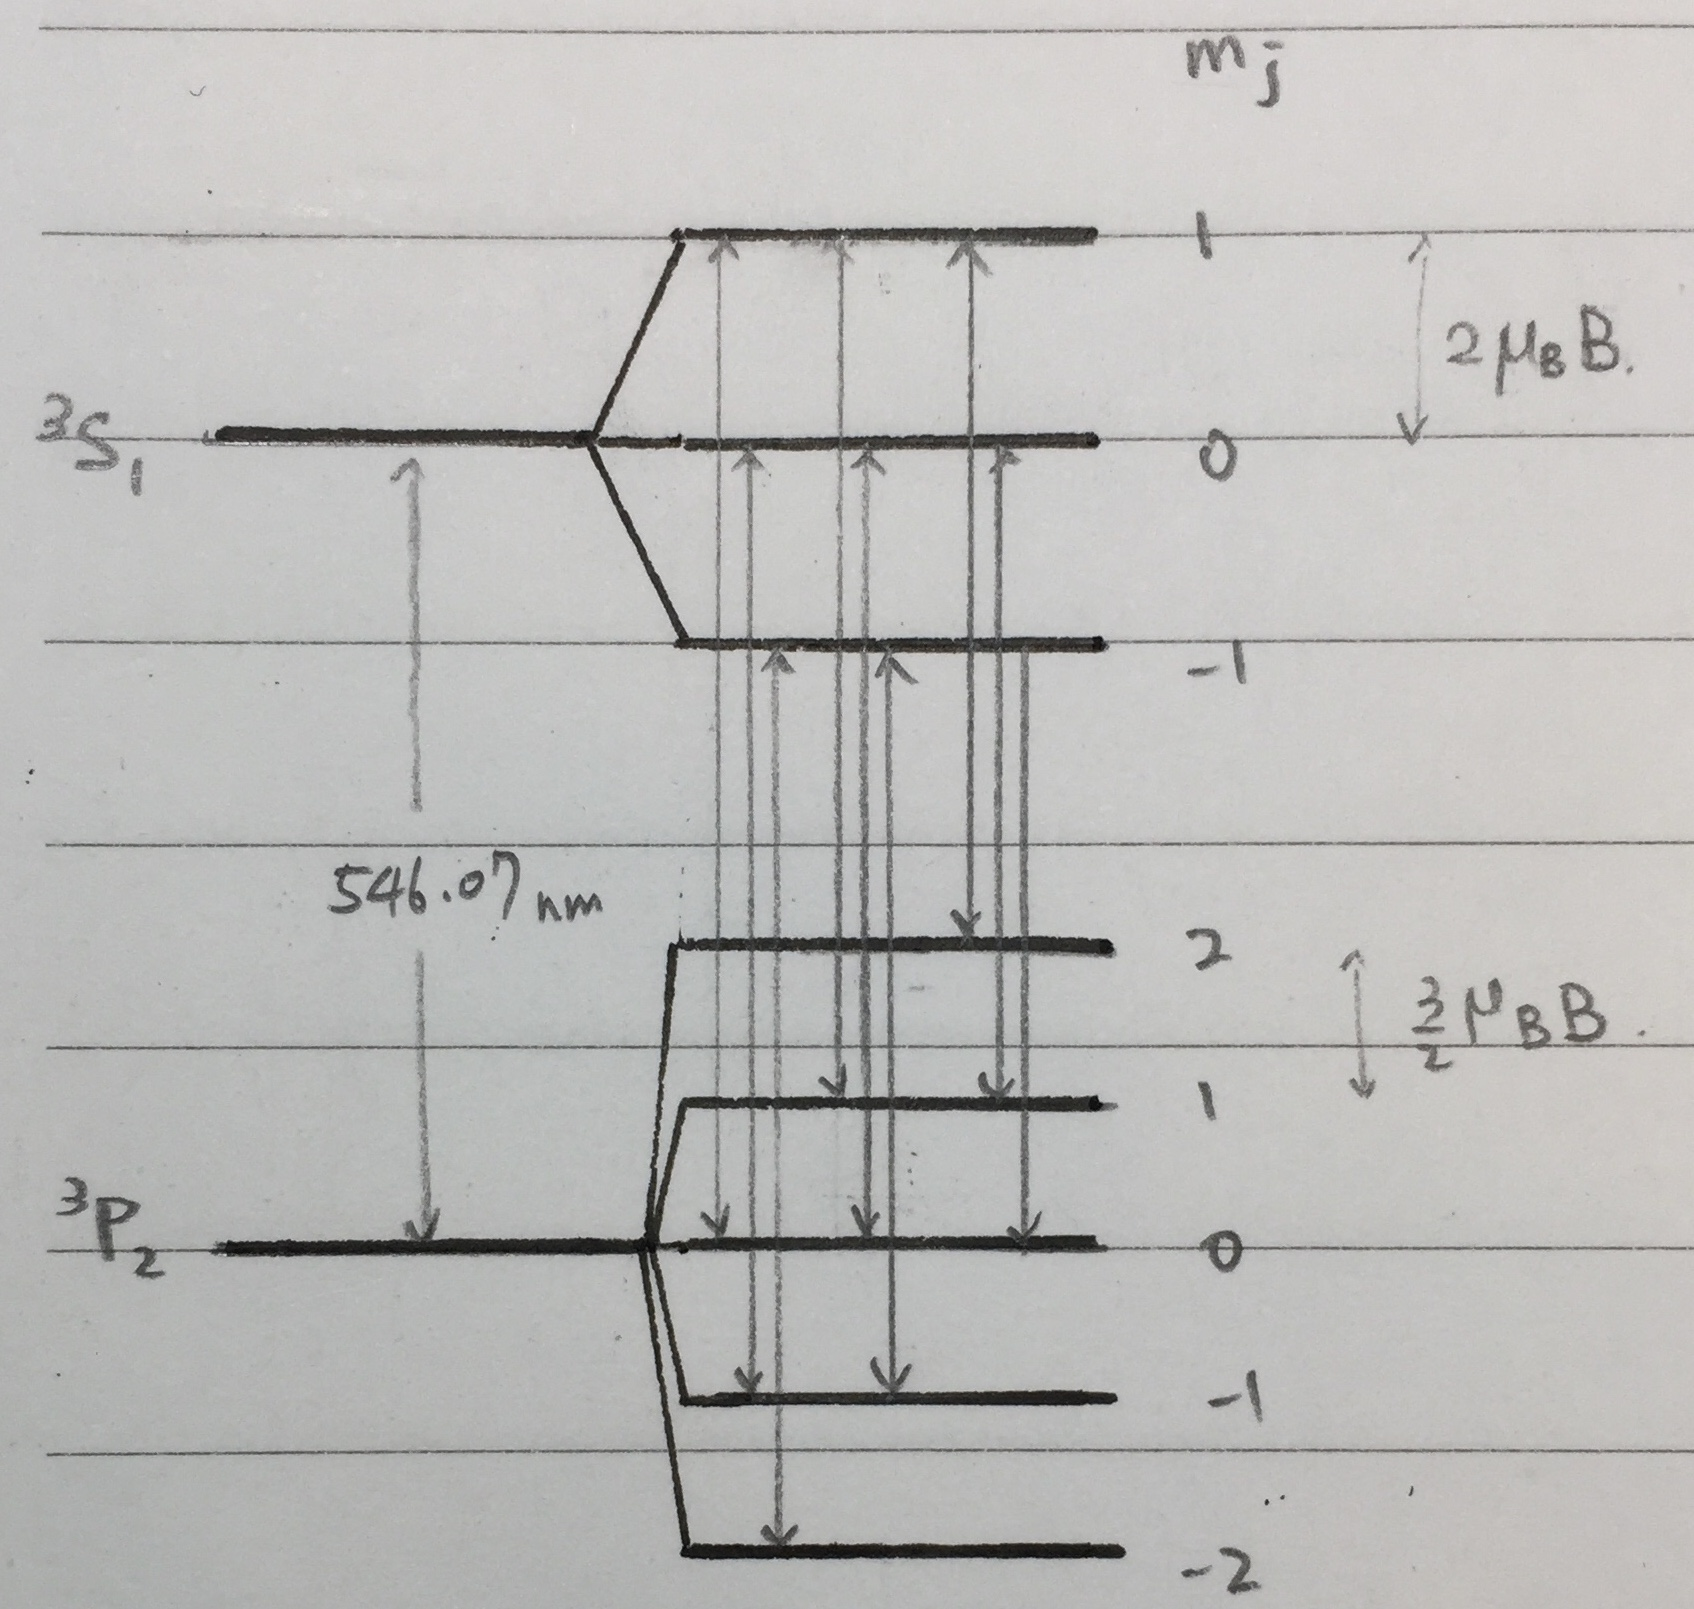
\includegraphics[width=5.3cm]{546nm}
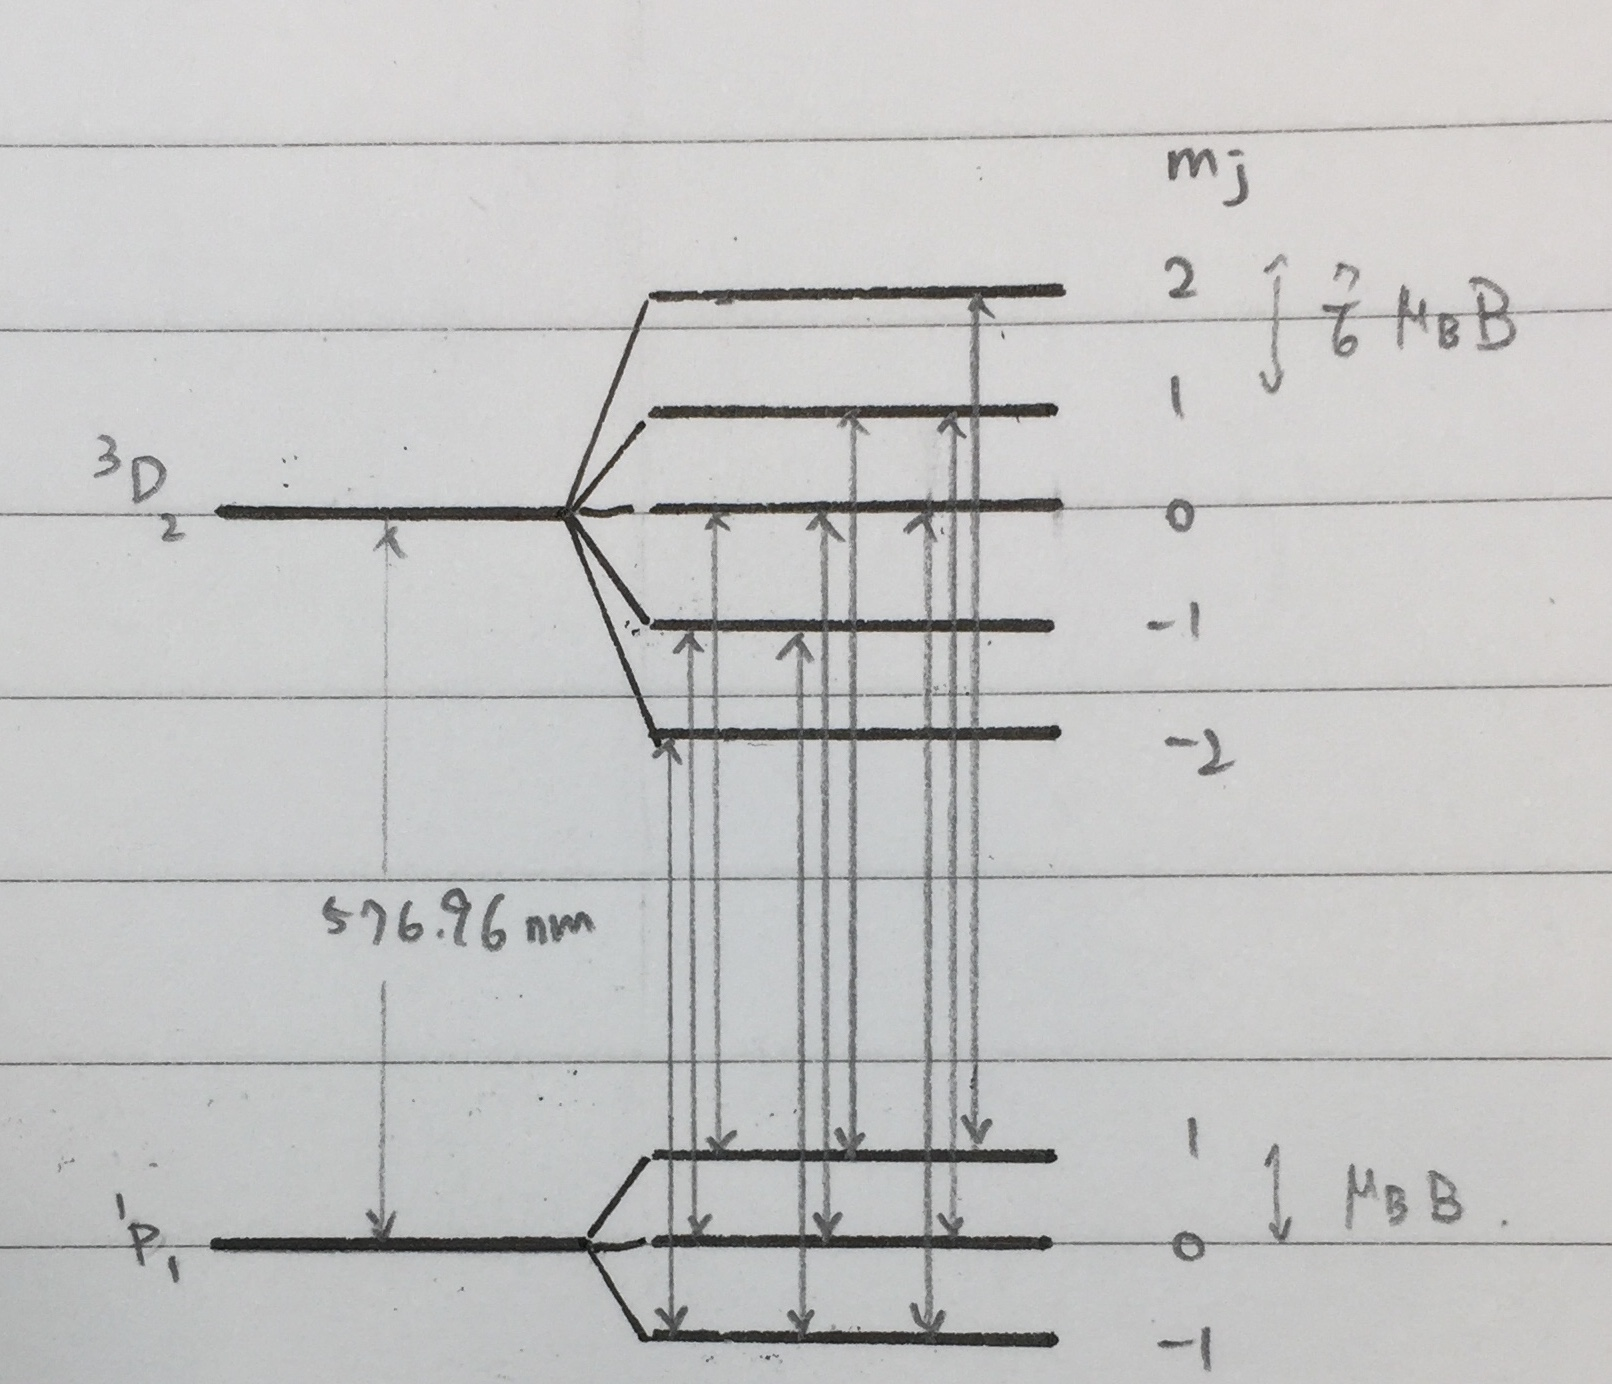
\includegraphics[width=5.3cm]{577nm}
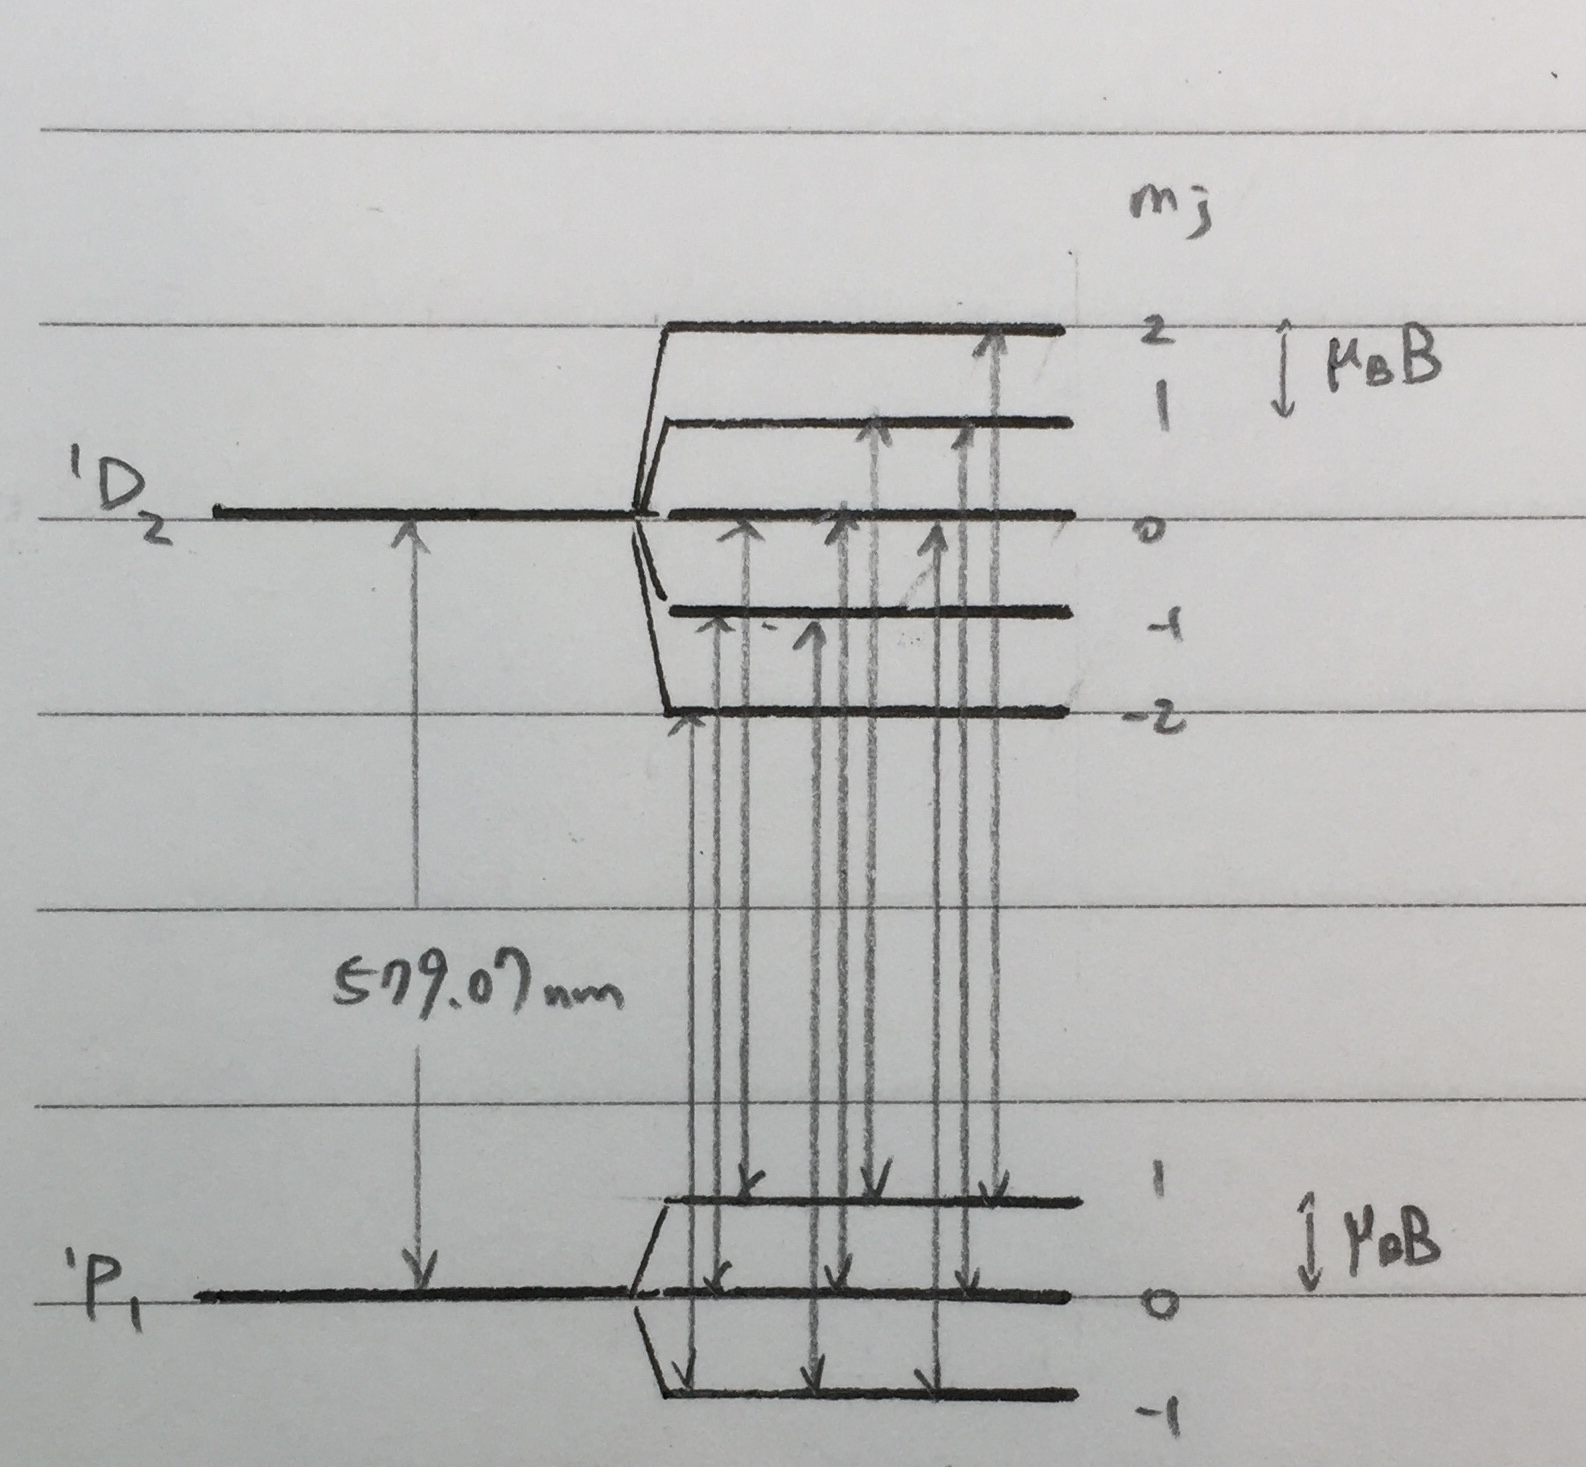
\includegraphics[width=5.3cm]{579nm}
\label{Fig. 1}
\caption{Energy level diagrams showing how the levels split under B field for the 546.07 nm green transition (left), 577 nm (middle) and 579 nm (right) yellow transitions. The arrows between splitted level represent possible transition, taking consideration of the selection rule.}
\end{figure}

\textbf{3. \textit{Comparison between theory and experiment}}
\smallskip

Because of the Zeeman effect, the transition energy between two levels in mercury is no longer just one single value. To calculate the change in transition energy between two levels when the B field is present, we can use Eq. (6) to find that 
$$ \Delta E_{magnetic} = (g_{Ji} m_{Ji} - g_{Jf} m_{Jf}) \mu_B B $$

From the energy level shifts calculated in section 2, it could be found that the $\Delta E_{magnetic}$ (in units of $\mu_B B$) has the following values for each transition:
\begin{align*}
\textbf{Green: }& 546.07 \text{ nm}: \Delta E_{magnetic} = -2, -1.5, -1, -0.5, 0, 0.5, 1, 1.5, 2 \\
\textbf{Yellow: }&576.96 \text{ nm}: \Delta E_{magnetic} = -\frac{8}{6}, -\frac{7}{6}, -1, -\frac{1}{6}, 0, \frac{1}{6}, 1, \frac{7}{6}, \frac{8}{6} \\
& 579.07 \text{ nm}: \Delta E_{magnetic} = -1, 0 ,1
\end{align*} 
Fig. 2 organized the theoretical values and the experimental ones in one table for easy comparison. Notice for $\lambda =577nm$ transition, there are only three experimental values instead of nine. This is because the nine theoretical values form three groups of spectral lines (i.e the first three, middle three, and the last three), and within each group, three spectral lines space very close together (an energy separation of only $\mu_B B /6$). Our equipment is unable to identify this small difference in wavelength, hence, seeing each group as one single spectral line.

As seen from the table, the measured value and theoretical values agree very well with each other. Even though some theoretical values do not lies within the uncertainty of the experimental ones, their differences are still within $0.15 \mu_B B$.


\begin{figure}[H]
\begin{center}
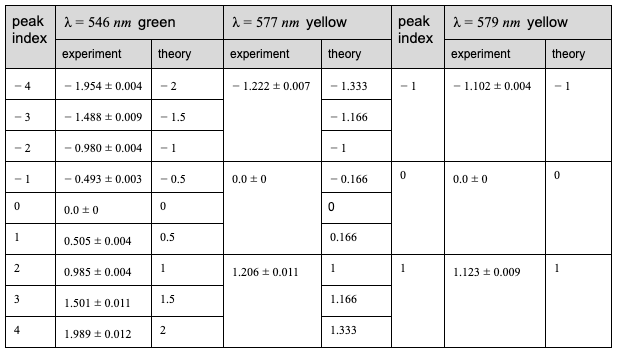
\includegraphics[width=15cm]{energies}
\label{Fig. 2}
\caption{Table showing the measured energy shifts and theatrically calculated energy shifts. }
\end{center}
\end{figure}
 
\end{document}